\subsection{Discretização da equação do calor}
\label{cap_discretizacao_equacao_calor}

Nesta seção, aborda-se a discretização da equação do calor utilizando-se o método dos volumes finitos com o diagrama de Voronoi. Também mostra-se um pseudocódigo referente a esse método.

\subsubsection{Considerações iniciais}

No método dos volumes finitos (MVF), o domínio do problema é dividido em um conjunto finito de volumes, adjacentes entre si, chamados de volumes de controle (VC). Nesse método, realiza-se um balanço de conservação da propriedade em questão, para cada volume elementar, de modo a se obter a equação aproximada, respeitando-se a lei de conservação. Há interesse na aplicação do método dos volumes finitos na solução de equações diferenciais parciais (EDPs) devido a essa característica.

Uma forma de se obter as equações aproximadas no MVF é integrar, sobre cada volume elementar, no espaço e no tempo, as equações na forma conservativa, ou divergente. Nessa forma, os termos relacionados aos fluxos aparecem dentro das derivadas em relação às coordenadas espaciais. Ao realizar a integração para todos os VCs, obtém-se uma equação algébrica para cada volume e, consequentemente, obtém-se um sistema de equações algébricas. Esse sistema de equações é formado pelas variáveis localizadas nos centróides dos VCs. Para as aproximações, utilizam-se funções de interpolação por meio dos valores das variáveis dos VCs vizinhos. Devido a sua generalidade, qualquer tipo de malha pode ser utilizada, regular ou irregular \cite[p. 27 - 33]{Maliska2010}.

Na seção (\ref{cap_equacao_calor}), apresenta-se o modelo matemático para difusão de fluidos. Na seção (\ref{cap_discretizacao_malha_irregular}), é tratada a discretização da equação do calor com o diagrama de Voronoi e apresenta-se o pseudocódigo dessa discretização.

\subsubsection{Equação do calor}\label{cap_equacao_calor}

A equação do calor é um modelo matemático para a difusão de calor em sólidos, ou seja, descreve o fluxo de calor em um corpo sólido. Esse modelo consiste em uma equação de derivadas parciais que, muitas vezes, é também chamada de equação de difusão. Essa equação, em sua forma generalizada, é definida como

\begin{equation}
\frac {\partial } {\partial t} (\rho \phi)  =  \nabla \cdot \left( \frac {k} {c_{p}} \nabla \phi \right) ,
\label{equacao_diferencial_calor_forma_geral}
\end{equation}

\noindent em que $\phi$ é a temperatura, $t$ é o tempo, $\rho$ é a massa volumétrica do material, $c_{p}$ é o seu calor específico e $k$ é a condutibilidade térmica. 

Segundo \citeonline[p. 73]{Tannehill1997}, pode-se integrar a equação (\ref{equacao_diferencial_calor_forma_geral}) sobre um volume $V$ qualquer obtendo-se

\[
\iiint_V  \left ( \frac {\partial } {\partial t} (\rho \phi)  +  \nabla \cdot {\mathbf q} \right )dV = 0,
\]
\noindent com ${\mathbf q} =  - \frac {k} {c_{p}} \nabla \phi$. Aplicando-se o teorema de Gauss, tem-se

\[
 \iiint _{V}   \frac {\partial } {\partial t} (\rho \phi) dV  +   \oiint_{S} {\mathbf q} \cdot {\mathbf n}  dS = 0.
\]

O ``volume'' contém uma unidade de profundidade em problemas bidimensionais. Nesse caso, ${\mathbf n} dS$ pode ser representado por $i dy - j dx$ para um caminho de integração na fronteira em sentido horário. Essa equação segue a lei de conservação. O primeiro termo na equação, uma integral sobre o volume, significa a taxa de variação da energia armazenada no volume em função do tempo. O segundo termo é uma integral de linha sobre a superfície do volume e representa a vazão de energia ao longo da superfície do volume na unidade de tempo \cite[p. 72 - 76]{Tannehill1997}. 

\subsubsection {Discretização da equação do calor com o diagrama de Voronoi}\label{cap_discretizacao_malha_irregular}

Nesta seção, é tratada a  discretização da equação do calor (\ref{equacao_diferencial_calor_forma_geral}) com o diagrama de Voronoi. Uma partição do diagrama de Voronoi pode ser vista na figura (\ref{fig_malha_voronoi}), na página \pageref{fig_malha_voronoi}. Esta discretização baseia-se no capítulo 13 de \citeonline[p. 322 - 385]{Maliska2010} e no capítulo 8 de \citeonline[p. 243 - 266]{Versteeg2007}.

Na figura (\ref{fig_volume_controle_integracao}), mostra-se o volume elementar com centróide $P$, sobre o qual será realizada a integração, e o VC adjacente, com centróide $Nb_{i}$. A equação discretizada é obtida integrando-se a equação (\ref{equacao_diferencial_calor_forma_geral}) em cada VC, no intervalo de tempo de $t$ a $t+ \Delta t$. 

\begin{figure}[!ht]
  \centering
  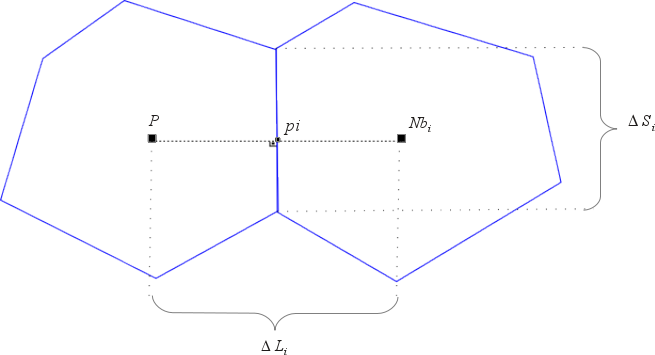
\includegraphics[width=200pt]{imagens_discretizacao/volume_controle_integracao.png}
  \caption{\footnotesize{Volumes de controle para a integração.
}}
  \label{fig_volume_controle_integracao}
\end{figure}

Integrando-se a equação (\ref{equacao_diferencial_calor_forma_geral}) no tempo e no espaço e adotando-se uma formulação implícita, obtém-se $
 \int_{t}^{t+ \Delta t}\int_{V} \frac {\partial} {\partial t} (\rho \phi) dV dt = \int_{t}^{t+ \Delta t} \int_{V} \nabla \cdot \left( \frac { k } { c_{p} } \nabla \phi \right) dV dt.$ O ponto de integração $pi$ localiza-se no ponto médio da interface dos polígonos com centróides $P$ e $Nb_{i}$. Aplicando-se o teorema da divergência e utilizando-se uma aproximação linear, tem-se

\begin{equation}
 \frac { M_{P}^{t + \Delta t} \phi_P^{t + \Delta t} - M_{P}^{t} \phi_{P}^{t} } { \Delta t} = \sum_{i=1}^{n} \left( \frac {k} {c_P} \left( \phi_{Nb_{i}}^{t + \Delta t} - \phi_{P}^{t + \Delta t} \right) \frac {\Delta S_{i}} {\Delta L_{i}} \right),
 \label {discretizacao_equacao_calor_1}
\end{equation}

\noindent em que $M_{P}=\rho \cdot A$ é a massa dentro do volume de controle e $A$ é a área do polígono com centróide $P$. $\phi_{P}$ é a temperatura do volume de controle com centróide $P$, $\phi_{Nb_{i}}$ é a temperatura no volume de controle com centróide $Nb_{i}$ e $n$ é o número de VCs adjacentes ao VC com centróide $P$. $\Delta S_i$ é o tamanho da interface entre os polígonos com centróide $P$ e seu polígono adjacente com centróide $Nb_i$ e $\Delta L_i$ é a distância entre os pontos $P$ e $Nb_i$. A equação (\ref{discretizacao_equacao_calor_1}) pode ser escrita como

\begin{equation}
 A_{P} \phi_{P}^{t+ \Delta t} - \sum_{i=1}^{n} A_{Nb_{i}} \phi_{Nb_{i}}^{t+ \Delta t} = B,
 \label{equacao_discretizacao_pologono_voronoi} 
\end{equation}

\noindent em que $A_{Nb_{i}} =  \frac{k} {c_{p}}  \cdot \frac {\Delta S_{i}} {\Delta L_{i}},  A_{P} = \sum_{i=1}^{n} A_{Nb_{i}} + \frac { M_{P}^{t+ \Delta t} } { \Delta t}$ e $B = \frac {M_{P}^{t} \phi_{P}^{t}} { \Delta t}.$

Caso um ou mais VCs adjacentes ao VC com centróide $P$ esteja localizado na fronteira e considerando-se condições de contorno de Dirichlet, a abordagem é da mesma forma que a empregada na seção anterior. Na aproximação linear da derivada na interface que separa o volume de controle com centróide $P$ e um volume de controle com centróide $F$, localizado na fronteira e adjacente ao VC com centróide $P$, terá o valor da temperatura de $F$ substituído pelo valor prescrito da condição de contorno. Os coeficientes $A_{Nb_{i}}$, $A_{P}$ e $B$ variam de acordo com a quantidade de VCs adjacentes localizados na fronteira. Com um centróide $F_{i}$ de um VC na fronteira, conforme pode ser visto na figura (\ref{fig_volume_controle_integracao_fronteira}), $\Delta S_{F_{i}}$ é o mesmo que $\Delta S_{i}$, ou seja, é o tamanho da interface entre os polígonos com centróide $P$ e seu polígono adjacente com centróide $F_i$ e $\Delta L_{F_{i}}$ é o mesmo que $\Delta L_{i}$, ou seja, é a distância entre os pontos $P$ e $F_i$. 

\begin{figure}[!ht]
  \centering
  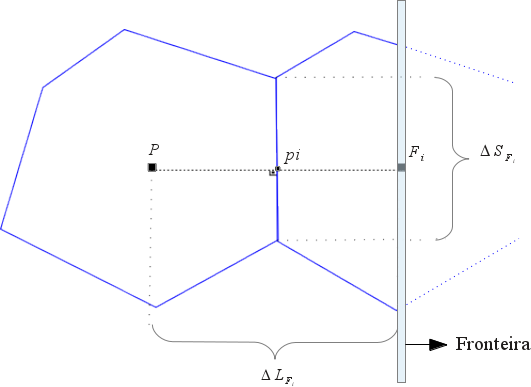
\includegraphics[width=180pt]{imagens_discretizacao/volume_controle_integracao_fronteira.png}
  \caption{\footnotesize{Volumes de controle para a integração com vizinho localizado na fronteira.
}}
  \label{fig_volume_controle_integracao_fronteira}
\end{figure}

A seguir, mostra-se um exemplo para ficar clara a forma com que se aplica o método dos volumes finitos com o diagrama de Voronoi nas ocorrências em que um VC contém VCs adjacentes na fronteira. Considere o volume de controle com  centróide $P_3$ mostrado na figura (\ref{fig_volume_voronoi_fronteira}). Os volumes adjacentes ao VC com centróide $P_3$, internos ao domínio, têm centróides $Nb_1$, $Nb_2$ e $Nb_3$ e os volumes  adjacentes ao VC com centróide $P_3$, localizados na fronteira, contêm valores prescritos e descritos nos pontos $F_1$, $F_2$ e $F_3$, $m_1$ é o número de volumes internos e adjacentes ao VC com centróide $P$, $m_2$ é o número de volumes de fronteira e adjacentes ao VC com centróide $P$ e $n = m_1 + m_2$.
Os valores das temperaturas nesses pontos são representados por $\phi_{F_{j}}$. Realizando-se a discretização da equação do calor para um volume localizado na fronteira, a equação (\ref{discretizacao_equacao_calor_1}) torna-se

\begin{figure}[!ht]
  \centering
  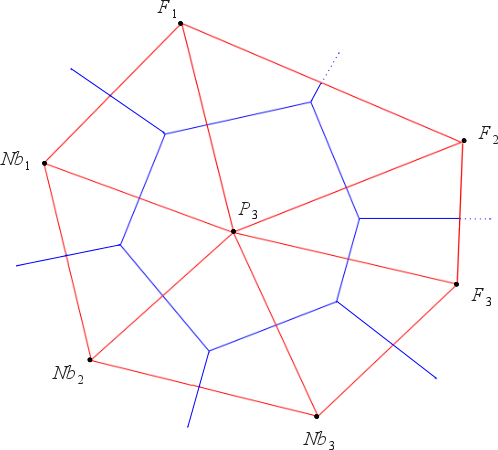
\includegraphics[width=150pt]{imagens_discretizacao/volume_voronoi_fronteira.png}
  \caption{\footnotesize{Volume de Voronoi adjacente a VCs com centróides localizados na fronteira. $Nb_1$, $Nb_2$ e $Nb_3$ são os centróides dos VCs internos ao domínio e $F_1$, $F_2$ e $F_3$ contêm valores prescritos em pontos localizados na fronteira.
}}
  \label{fig_volume_voronoi_fronteira}
\end{figure}


\begin{eqnarray}
 \frac { M_{P}^{t + \Delta t} \phi_P^{t + \Delta t} - M_{P}^{t} \phi_{P}^{t} } { \Delta t} &=& \sum_{i=1}^{m_1} \left( \frac {k} {c_P} \left( \phi_{Nb_{i}}^{t + \Delta t} - \phi_{P}^{t + \Delta t} \right) \frac {\Delta S_{i}} {\Delta L_{i}} \right) \nonumber \\
 & & + \sum_{i=1}^{m_2} \left( \frac {k} {c_P} \left( \phi_{F_{i}}^{t + \Delta t} - \phi_{P}^{t + \Delta t} \right) \frac {\Delta S_{F_{i}}} {\Delta L_{F_{i}}} \right), \nonumber
\end{eqnarray}

\noindent que pode ser reescrita como

\begin{equation}
 A_{P} \phi_{P}^{t+ \Delta t} - \sum_{i=1}^{m_1} A_{Nb_{i}} \phi_{Nb_{i}}^{t+ \Delta t}  = B,
 \label{equacao_discretizacao_pologono_voronoi_fronteira} 
\end{equation}

\noindent em que $A_{Nb_{i}} = \left( \frac{k} {c_{p}}  \frac {\Delta S_{i}} {\Delta L_{i}} \right), A_{F_{i}} = \left( \frac{k} {c_{p}}  \frac {\Delta S_{F_{i}}} {\Delta L_{F_{i}}} \right), A_{P} = \sum_{i=1}^{m_1} A_{Nb_{i}} + \sum_{i=1}^{m_2} A_{F_{i}} + \frac { M_{P}^{t+ \Delta t} } { \Delta t}, B = \frac {M_{P}^{t} \phi_{P}^{t}} { \Delta t} + \sum_{i=1}^{m_2} A_{F_{i}} \phi_{F_{i}}^{t+ \Delta t}$. Dessa forma, tem-se a discretização da equação do calor com polígonos de Voronoi.

A seguir, no algoritmo \ref{algoritmo_metodo_volumes_finitos}, é apresentado um pseudocódigo referente à discretização da equação do calor com polígonos de Voronoi, mostrado na figura (\ref{fig_malha_voronoi}). Um sistema de equações lineares é gerado, em que a equação de cada VC da malha, interno ao domínio ou localizado na fronteira é, respectivamente, conforme a equação (\ref{equacao_discretizacao_pologono_voronoi}) ou conforme a equação (\ref{equacao_discretizacao_pologono_voronoi_fronteira}).  No pseudocódigo, os valores dos coeficientes são armazenados em objetos que representam os vértices da triangulação de Delaunay. 

\begin{algorithm}
\caption{ Método dos volumes finitos.} 
\label{algoritmo_metodo_volumes_finitos}
\Entrada{lista dos v\'ertices da triangula\c{c}\~ao de Delaunay.}
\Saida{lista dos v\'ertices da triangula\c{c}\~ao de Delaunay com os coeficientes $A_{P}$, $A_{Nb_{i}}$ e $B$ preenchidos.}
\Inicio{
  \ParaCada{ ( v\'ertice interno P da triangula\c{c}\~ao de Delaunay) } 
  {
    \CommentSty{ // $Area_{P}$ é a \'area do VC com centr\'oide $P$}\\     
    $P.A_{P} \leftarrow \frac { \rho \cdot Area_{P} } { \Delta t};$  
    $P.B \leftarrow \frac { \rho \cdot Area_{P} } { \Delta t} \cdot P.valorTemperaturaEtapaAnterior;$\\
    \ParaCada{( v\'ertice $Nb_i$ adjacente a $P$)} {
      $P.A_{Nb_{i}} \leftarrow 0;$ \\ 
      \uSe { (v\'ertice $Nb_{i}$ localiza-se na fronteira)} {         
	\CommentSty{// $\Delta S_{F_{i}}$ e $\Delta L_{F_{i}}$ são calculados conforme\\ // mostrado na fig.(\ref{fig_volume_controle_integracao_fronteira})} \\           
	$P.A_{P} \leftarrow P.A_{P} +  \frac{k} {c_{p}}  \frac {\Delta S_{F_{i}}} { \Delta L_{F_{i}} };$ \\          
	\CommentSty{// $valorTemperatura$ \'e definida pelas\\ // condi\c{c}\~oes de contorno}\\     
	$P.B \leftarrow P.B + ( Nb_{i}.valorTemperatura \cdot \frac{k} {c_{p}}  \frac {\Delta S_{i}} { \Delta L_{i} });$ \\
	\CommentSty{// $Nb_{i}$ localiza-se na fronteira,\\ // portanto $F_{i} = Nb_{i}$  }\\           
      }\Senao {
	\CommentSty{// $\Delta S_{i}$ e $\Delta L_{i}$ são calculados conforme\\ // mostrado na fig. (\ref{fig_volume_controle_integracao})} \\           
	$P.A_{P} \leftarrow P.A_{P} +  \frac{k} {c_{p}}  \frac {\Delta S_{i}} { \Delta L_{i} };$ \\          
	$P.A_{Nb_{i}} \leftarrow P.A_{Nb_{i}} - \frac{k} {c_{p}} \frac {\Delta S_{i}} { \Delta L_{i} };$\\
      }
    }
  }
}
\end{algorithm}

\subsubsection{Resumo}

Nesta seção, abordou-se a discretização da equação do calor. Primeiramente, na subseção (\ref{cap_equacao_calor}), apresentou-se o modelo matemático que descreve a difusão de calor em sólidos. 
Na subseção (\ref{cap_discretizacao_malha_irregular}), utilizou-se o MVF com o diagrama de Voronoi. Por fim, apresentou-se um pseudocódigo referente a essa discretização.